\subsection{Credit Risk Management CR-3}






Chapter 16、17 和 18 都是关于信用风险的管理

* Chapter 16: 站在银行贷款的角度管理风险，更多的涉及的是规章制度。

* Chapter 17: 站在持有 bond 的角度， 用信用衍生品， 管理 bond 投资带来的信用风险。

* Chapter 18: 站在银行资产[各种 loan、mortgage 等]角度， 采取证券化手段把这些有风险资产转嫁出去。

【本节知识点， 站在银行贷款的角度管理风险。】

\begin{itemize}
\item Key Elements of Effective Lending/Financing Policy
\end{itemize}

 Credit facility scope and allocation: 明确规定银行的信贷业务范围，包括哪些类型的贷款和融资产品可以提供， 涵盖的客户群体， 以及允许的最大敞口限额。

Credit portfolio management 信贷组合管理

信贷风险管理的全过程， 包括贷款的 origin、评估 (appraisal)、内部监督 (internal supervision) 和收款程序 (collection procedures)。

强调在每个阶段如何识别、评估和管理风险，确保在整个贷款生命周期中对风险的持续控制和监管。

Emphasize non-restrictiveness and flexibility 强调非限制性和灵活性

强调政策的灵活性， 使其能够适应市场和经济环境的变化。银行应能够根据新的风险和市场条件及时调整其信贷策略。

 符合监管机构对信贷政策的最低标准要求。

 董事会和高级管理层的参与

 风险分类和损失准备金

包括将资产按信贷风险敞口和可收回性分类，以及为潜在损失建立拨备的具体方法和标准。

Setting Exposure and Concentration Limits

监管机构通常关注三个领域:

\begin{itemize}
\item 对单一客户的敞口 exposure to a single customer
\end{itemize}

\begin{itemize}
\item 关联方融资 related-party financing
\end{itemize}

3 对某一经济部门或地理区域的过度敞口 over exposure to an economic sector or geographic area。

/ Concentration limits 集中度限制:指的是对单一客户、地区或经济部门的最大敞口。银行通常根据准备金或资本的百分比设定限制

 Related parties 关联方可能会对银行的信贷决策产生控制作用。关联方包括母公司、子公司、主要银行股东、关联公司、董事和高级管理人员。

\begin{itemize}
\item Credit Facility Allocation and Credit Risk Reduction: 银行在制定和执行贷款政策时需要考虑的关键因素
\end{itemize}

A Lending authority 贷款授权:贷款政策应设定贷款官员的授权限制。有经验或任期较长的贷款官员可能会有更高的限额。

在小型银行通常是集中化的， 而在大型银行则可能根据地理区域、 贷款产品或客户类型进行分散化授权。

Types and distribution of loans 贷款类型和分布

通常对商业、房地产、消费者等贷款类别设定限制，并且任何超出限制的行为应得到董事会的批准。

Appraisal process 评估过程

 贷款定价 Loan pricing: 贷款利率应根据资金成本、贷款监督和行政开支的结构。应考虑损失概率和银行的合理利润率。

 Maturities 到期期限:贷款政策应为各种贷款类型设定明确的最大到期期限。

\begin{itemize}
\item Exposure to geographic or sector-level concentration 地理或行业集中度风险
\end{itemize}

 Availability of current financial information 当前财务信息的可用性:贷款政策应明确规定商业和消费者贷款所需的财务信息。

\begin{itemize}
\item Monitoring of collections 催收监控
\end{itemize}

 Limits on total loans outstanding 总贷款余额限制:贷款政策应设定关于总贷款余额的限制。

A Maximum ratio of loans to market value of pledged securities 质押证券市值与贷款最大比率:应为所有抵押品类型明确设定保证金要求。

Impairment recognition 贷款减值确认:应定期系统地识别贷款减值

 Renegotiated debt treatment 重组债务处理

V Written internal guidelines 书面内部指导方针: 所有贷款政策都应有适当的文件记录，不能仅靠口头理解。

\begin{itemize}
\item Credit Asset Classification 信贷资产分类
\end{itemize}

 资产分类是根据偿还可能性将银行资产分配到信用风险评级的过程，是信贷风险管理的关键工具。类别:

 Standard， or pass 标准/及格: 无逾期问题， 有充分现金或等值现金担保

♤ Specially mentioned， or watch 特别提及/观察:存在影响借款人偿还能力的弱点

 Substandard 次级: 具有明确的还款弱点， 可能危及偿还。

 Doubtful 可疑: 与次级相似但预期损失更为明显

Collection in full is questionable

 Loss: 偿还迟滞相对确定， 准备核销

Nonperforming Loans analysis 不良贷款分析

 Aging of past-due loans 逾期时间

\begin{itemize}
\item Reasons for the deterioration of loan portfolio quality
\end{itemize}

Case-by-case assessment of a list of nonperforming loans 单独审查每个逾期案例

 Provision levels 准备金水平

Loan Loss Provisions and Loan Loss Reserves

Loan Loss Provisions 贷款损失准备金

Specific amounts set aside by a bank for potential losses on loans.

考虑因素: like credit policies， prior loss experiences， and economic conditions

Loan Loss Reserves 贷款损失储备

Not assigned to specific assets

General reserves counted as Tier 2 capital， used to absorb unexpected losses. 作为二级资本的一部分， 用于吸收意外损失

Loan loss provisions cover specific amounts， while reserves are general and form part of the bank's capital structure.


\subsection{Credit Derivatives CR-13}




金融机构可以使用信用衍生品管理信用风险。本章节主要涉及 CDS、TRS。 【关于 CDS 相关知识点， 在 FRM 一级以及二级其他科目都或多或少的有所涉及， 这里做一个相对全面的介绍。CDS 是本科目重要知识点。】

1. Credit default swap 信用违约互换

(1) 基本概念

一个典型的例子:

一个投资者 \(\mathrm{A}\) 买了一个 \(\mathrm{C}\) 公司发行的债券，但是担心 \(\mathrm{C}\) 公司未来违约(信用风险)， 然后向一家 B 金融机构购买了一个 “保险”， 提供的保护就是关于公司 \(\mathrm{C}\) 是否违约。

 零时刻或者特定时刻:投资者 A 向金融机构 B 支付保费

未来:如果公司 C 违约，投资者 A 虽然不能收到来自公司 C 的资金， 但是因为购买了 “保险”， 金融机构 B 将会对此进行 “保险” 赔付。

这里的 “保险” 就是我们将要介绍的 CDS。

\begin{itemize}
\item A credit default swap 信用违约互换 (CDS) is a derivative contract between two parties， a credit protection buyer and credit protection seller， in which the buyer makes a series of cash payments to the seller and receives a promise of compensation for credit losses resulting from a credit event in an underlying.
\end{itemize}

\begin{itemize}
\item Credit default swaps (CDS) is essentially an insurance contract for the reference， the reference obligation is the fixed income security on which the swap is written-usually a bond but potentially also a loan.
\end{itemize}

\begin{itemize}
\item 与保险很像，与 put option 类似
\end{itemize}

\begin{center}
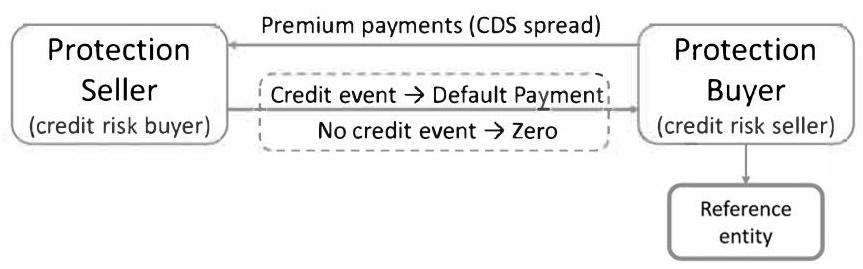
\includegraphics[width=0.7\textwidth]{images/0196660e-d86d-7ef6-8951-a48e2a482302_49_306_1566_863_269_0.jpg}
\end{center}
\hspace*{3em} 

\begin{itemize}
\item CDS 用作风险管理
\end{itemize}

如果持有一个有风险的债券，买一个 CDS，相当于将债券的风险转移出去， 进而相当于购买了无风险债券进行风险管理。

 一个有风险的公司债的多头相当于无风险债券的多头再卖出一份 CDS。



\[
{\text{ Bond }}_{\text{ risky }} + \mathrm{{CDS}} = {\text{ Bond }}_{\text{ risk free }}
\]

\[
{\text{ Bond }}_{\text{ risky }} = {\text{ Bond }}_{\text{ risk free }} - \text{ CDS }
\]



【这是个理念性公式。这个公式在以前的原版书上是有的， 现在没了。我感觉很好， 笔记就保留了下来】

Y 另外有 CDS 可以只管理信用风险，并不能管理市场风险，这不同于后面学习的总收益互换。但同时 CDS 还会引入新的信用风险，即 CDS 的卖方可能违约。

\begin{itemize}
\item 交易方:
\end{itemize}

credit protection buyer=the buyer of CDS(CDS 买方， 保护的买方， 风险的卖方)=short position of CDS

 例如上述例子中的投资者 \(\mathrm{A}\) 。

 支付一定的保费 fee/premium(可能是期初一次支付， 也可以是后期定期支付)。如果标的资产违约， CDS 卖出方给予买方一定的赔付。如果标的资产没有违约，白白支付了 premium。

 注意: 风险的卖方， 因此也称 short position of CDS (受益于受益于标的资产信用质量的恶化，也就是风险变大)。

credit protection seller=the seller of CDS(CDS 卖方， 保护的卖方， 风险的买方)=long position of CDS

 例如上述例子中的金融机构 \(\mathrm{B}\) 。

 收取一定保费。如果标的资产违约，给予买方一定的赔付。如果标的资产不违约，白白获得 premium。

 注意: 风险的买方， 因此也称 long position of CDS (受益于标的资产信用质量的好转， 也就是风险变小)。

注意: 在 CDS 这里， long CDS 意味着是 credit protection seller; short CDS 意味着 credit protection buyer。这与其他衍生品不同，这里可做特殊记忆。

\begin{itemize}
\item Reference entity 参考实体:
\end{itemize}

也就是债券的发行人。类似例子中的 C 公司

 reference obligation 参考债务/参照资产:发行人发行的(一个或多个)债务工具(bond/loan)

\begin{itemize}
\item Notional amount/principal:
\end{itemize}

 类似保险的保额

\begin{itemize}
\item The total face value of the bonds that can be sold is known as the credit default swap's notional principal. 【total face value of the bonds=CDS 的 notional principal \(\rbrack\)
\end{itemize}

 The amount of protection being purchased. 【最后的赔付是按照这个 Notional amount 来的】

\begin{itemize}
\item CDS spread 保费:the periodic premium that the buyer of a CDS pays to the seller for protection against credit risk.
\end{itemize}

 The protection buyer pays the seller a premium that is either paid upfront or over a period of time (一次性预交或定期支付).

类似上述例子中的:投资者 A 向金融机构 B 支付的保费

 CDS spread 也称 credit spread 信用利差。从概念上讲， 它与债券的信用利差相同，是承担信用风险的补偿。

 CDS spread 反映 reference obligation 的信用风险。

\begin{itemize}
\item CDS coupon rate (\%):
\end{itemize}

【在 CDS 的发展历史上， 最初 CDS 是非常定制化的， 因此， CDS spread 各异。随着 CDS 的发展， CDS 慢慢标准化。CDS coupon 是标准化的 CDS spread】

 标准化的 CDS spread， 也称 fixed coupon on CDS.

\(1\%\) for a CDS on an investment-grade company or index;

5\% for a CDS on a high-yield company or index.

投资级债券的 CDS coupon 为 1\%， 非投资级债券的 CDS coupon 为 5\%。【实际市场交易的 CDS 保费在此基础上进行调整】

CDS spread:市场定价

CDS coupon:标准化合约下的标准化保费支付

\begin{itemize}
\item Upfront premium \(\rightarrow\) The difference between the standardized coupon rate and the credit spread is paid upfront by one of the parties to the contract.【处理原则:期初一次性；多退少补】
\end{itemize}

若交易的 CDS spread 不是标准化的， 比如 CDS spread=3\%。

如果交易的是投资级的 CDS， 少交 2\%的 spread (本身需要支付 3\% 的保费，但是按照标准化合约，只支付 1\%，那么还少交了 2\%)。 那么保护的买方在期初一次性把所有差额补给保护的卖方。

如果交易的是投机级的 CDS，多交 2\%的 spread。那么保护的卖方在期初一次性退回所有差额给保护的买方。

Upfront premium 预付保费 (\%) \(\approx\) (Credit spread - Fixed coupon) \(\times\) Duration

Duration: CDS 的有效久期。题目通常会给定

Fixed coupon: 投资级是 1\%; 投机级是 5\%

例题: Assume a high-yield company's 10-year credit spread is 600 bps and the duration of the CDS is 8 years. What is the approximate upfront premium required to buy 10-year CDS protection? Assume high-yield companies have 5\% coupons on their CDS.

* Solution:upfront premium \(= \left( {6\%  - 5\% }\right)  * 8 = 8\%\)

\begin{itemize}
\item Credit Events 信用事件
\end{itemize}

这些信用事件发生，意味着债券发行人违约，也就是保护的卖方要赔付了。credit events 类型:【关于类型， 了解即可】

Bankruptcy 债券发行人破产

Failure to pay。还没有到破产程度， 但是未按计划支付

Restructuring 重组: 指一系列可能的事件， 包括减少或推迟本金或利息、债务优先级或顺位的变更等

 在美国，重组通常不被视为信用事件，因为破产通常是美国公司的首选路径。

 在美国以外的地区， 重组被视为信用事件。

(2) CDS 的结算

 physical settlement 实物结算【一手交钱(赔付)，一手交货(违约的债券)】 involves actual delivery of the debt instrument in exchange for a payment by the credit protection seller of the notional amount of the contract

也就是信用事件发生后， CDS buyer 把这个违约的债务工具 (Reference obligation)， 递交给 CDS seller。CDS seller 进行赔付 (Notional amount)。

\begin{center}
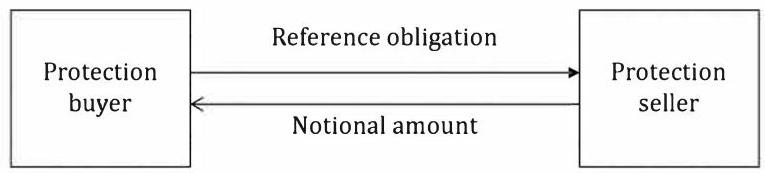
\includegraphics[width=0.6\textwidth]{images/0196660e-d86d-7ef6-8951-a48e2a482302_52_467_1657_765_173_0.jpg}
\end{center}
\hspace*{3em} 

实际市场中， CDS buyer 递交的这个债务工具是有一定选择范围的， 只要满足标准即可。这个选择叫做 cheapest deliverable bond。(如同一级学习的长期国债期货合约那样， 可以选择)

Cash settlement 现金结算

如果标的资产发生违约，信用违约互换的卖方会按照违约差价赔付

给买方，违约差价指的是资产的面值和违约发生后的价值之差。

\begin{center}
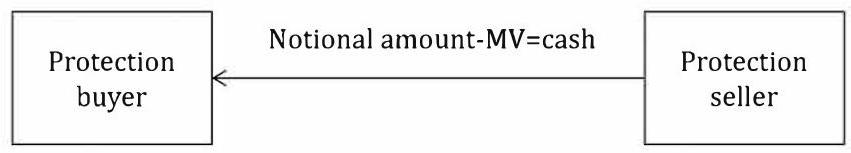
\includegraphics[width=0.7\textwidth]{images/0196660e-d86d-7ef6-8951-a48e2a482302_53_423_264_851_153_0.jpg}
\end{center}
\hspace*{3em} 

 Payout amount = Notional amount-债券回收的市场价值

(3) Pricing of CDS【这个知识学习性价比较低，会涉及大量计算。这里借由原版书例子给出】

\begin{itemize}
\item Pricing means determining the CDS spread or upfront payment given a particular coupon rate for a contract. 【定价定的是 CDS spread 或者 upfront payment。而我们这里主要指的是确定 CDS spread】
\end{itemize}

\begin{itemize}
\item accrual payment 应计支付: 在 CDS 定价中考虑应计支付
\end{itemize}

因为违约可能在一年中的任何时间发生，而保费支付通常年末。因此， 应计支付考虑了在支付期中途违约的情况下，投资者应获得的部分保护。 【类似于债券中的累计利息概念】

\begin{itemize}
\item 定价逻辑:
\end{itemize}

\(\checkmark \;\) CDS 买方支付的保费现值之和(没有违约和违约情况)=其收到的赔付现值之和

 CDS 买方支付的保费现值之和:Present Value of Expected Payments(没有违约)+the Present Value of Accrual Payment (违约情况下)

 CDS 买方收到的赔付之和: the Present Value of Expected Payoff

在这个原则下，计算 CDS spread。【这种分析方式类似，一级中的保险保费的计算】

\begin{itemize}
\item 说明:如果已知 CDS spread，可以求得违约概率。【见 “Estimating Default Probabilities from Credit Spreads" 】
\end{itemize}

\begin{itemize}
\item 原版书例子: 一个 5-year CDS
\end{itemize}

\begin{itemize}
\item Hazard rate of the reference entity: 2\% per annum
\end{itemize}

\begin{itemize}
\item Risk-free interest rate is 5\% per annum with continuous compounding
\end{itemize}

 Payments are made once a year at the end of each year.【保费在每年的期末支付】

\begin{itemize}
\item Notional principal of \(\$ 1\)
\end{itemize}

 Defaults happen halfway through a year【如果参考实体违约，假设发生中一年的年中】

 Recovery rate is 40\%【参考实体发行的债券回收率】

计算 CDS spread。(CDS spread 用 \(\mathrm{s}\) 表示)

\begin{itemize}
\item 分析:
\end{itemize}

 第一步:计算所需概率【利用违约强度模型】

\begin{center}
\adjustbox{max width=\textwidth}{
\begin{tabular}{|c|c|c|}
\hline
Year & Probability of surviving to year end & Probability of default during year \\
\cline{1-3}
1 & 0.9802 & 0.0198 \\
\cline{1-3}
2 & 0.9608 & 0.0194 \\
\cline{1-3}
3 & 0.9418 & 0.0190 \\
\cline{1-3}
4 & 0.9231 & 0.0186 \\
\cline{1-3}
5 & 0.9048 & 0.0183 \\
\cline{1-3}
\hline
\end{tabular}
}
\end{center}

Cumulative \(\mathrm{{PD}} = 1 - {\mathrm{e}}^{-\bar{\lambda }\mathrm{t}}\)

Cumulative survival rate \(= {\mathrm{e}}^{-\bar{\lambda }\mathrm{t}}\)

 例如: 第一年的生存概率=e \({}^{-{0.02} \times  1} = {0.9802}\)

 第二年的生存概率=e \({}^{-{0.02} \times  2} = {0.9608}\)

 第三年的生存概率 \(= {\mathrm{e}}^{-{0.02}^{ \times  }3} = {0.9418}\)

◇ 以此类推

 第一年的违约概率 \(= 1 - {0.9802} = {0.198}\)

 第二年的违约概率 \(= {0.9802} - {0.9608} = {0.0194}\)

/ 第二步， Calculation of the Present Value of Expected Payments [计算没有违约的情况下，支付的保费之和】

 只有在前面时间没有违约的情况下， 才会支付下一期的保费

\begin{center}
\adjustbox{max width=\textwidth}{
\begin{tabular}{|c|c|c|c|c|}
\hline
\multicolumn{5}{|c|}{Payment = s per annum.} \\
\cline{1-5}
Time (years) & Probability of survival & Expected payment & Discount factor & PV of expected payment \\
\cline{1-5}
1 & 0.9802 & 0.9802s & 0.9512 & 0.9324s \\
\cline{1-5}
2 & 0.9608 & 0.9608s & 0.9048 & 0.8694s \\
\cline{1-5}
3 & 0.9418 & 0.9418s & 0.8607 & 0.8106s \\
\cline{1-5}
4 & 0.9231 & 0.9231 s & 0.8187 & 0.7558s \\
\cline{1-5}
5 & 0.9048 & 0.9048s & 0.7788 & 0.7047 s \\
\cline{1-5}
Total & \phantom{X} & \phantom{X} & \phantom{X} & 4.0728s \\
\cline{1-5}
\hline
\end{tabular}
}
\end{center}

 例如:第一年的预期支付现值=生存概率×保费×贴现因子=0.9802 ×s × \({\mathrm{e}}^{-{0.05} \times  1} = {0.9802} \times  \mathrm{s} \times  {0.9512} = {0.9324}\mathrm{\;s}\)

 总现值: 所有年份的预期支付现值之和= 4.0728s。

 第三步， Calculation of the Present Value of Accrual Payment【计算有违约的情况下的支付】

 违约发生在每年年中，应计支付 \(= {0.5}\mathrm{s}\)

\begin{center}
\adjustbox{max width=\textwidth}{
\begin{tabular}{|c|c|c|c|c|}
\hline
Time (years) & Probability of default & Expected accrual payment & Discount factor & PV of expected accrual payment \\
\cline{1-5}
0.5 & 0.0198 & 0.0099s & 0.9753 & 0.0097 s \\
\cline{1-5}
1.5 & 0.0194 & 0.0097s & 0.9277 & 0.0090s \\
\cline{1-5}
2.5 & 0.0190 & 0.0095s & 0.8825 & 0.0084s \\
\cline{1-5}
3.5 & 0.0186 & 0.0093s & 0.8395 & 0.0078s \\
\cline{1-5}
4.5 & 0.0183 & 0.0091 s & 0.7985 & 0.0073s \\
\cline{1-5}
Total & \phantom{X} & \phantom{X} & \phantom{X} & 0.0422s \\
\cline{1-5}
\hline
\end{tabular}
}
\end{center}

 第一年的应计支付现值 \(=\) 违约概率 \(\times\) 应计支付 \(\times\) 贴现因子 \(=\)  \({0.0198} \times  {0.5}\mathrm{\;S} \times  {0.9753} = {0.0097}\mathrm{\;S}\)

 总现值: 所有年份的应计支付现值之和 \(= {0.0422}\mathrm{\;s}\) 。

/ 第四步:Calculation of the Present Value of Expected Payoff【赔付现值之和】

\begin{center}
\adjustbox{max width=\textwidth}{
\begin{tabular}{|c|c|c|c|c|c|}
\hline
\multicolumn{6}{|c|}{Notional principal \(=  + 1\) .} \\
\cline{1-6}
Time (years) & Probability of default & Recovery rate & Expected payoff (\$) & Discount factor & PV of expected payoff (\$) \\
\cline{1-6}
0.5 & 0.0198 & 0.4 & 0.0119 & 0.9753 & 0.0116 \\
\cline{1-6}
1.5 & 0.0194 & 0.4 & 0.0116 & 0.9277 & 0.0108 \\
\cline{1-6}
2.5 & 0.0190 & 0.4 & 0.0114 & 0.8825 & 0.0101 \\
\cline{1-6}
3.5 & 0.0186 & 0.4 & 0.0112 & 0.8395 & 0.0094 \\
\cline{1-6}
4.5 & 0.0183 & 0.4 & 0.0110 & 0.7985 & 0.0088 \\
\cline{1-6}
Total & \phantom{X} & \phantom{X} & \phantom{X} & \phantom{X} & 0.0506 \\
\cline{1-6}
\hline
\end{tabular}
}
\end{center}

 计算每年的预期回报现值: 【考虑每个违约情况】

例如: 第一年的预期回报现值 \(=\) expected payoff \(\times\) 贴现因子 \(= {0.0119}\)  \(\times  {0.9753} = {0.0116}\) 【这里在折现的时候，注意折现时间，是每年的年中， 折现因子这里已经体现。】

◆ 总现值=0.0506。

 最后:联立等式

\[
{4.0728}\mathrm{\;s} + {0.0422}\mathrm{\;s} = {0.0506} \rightarrow  \mathrm{s} = {0.0123}
\]

The mid-market CDS spread for the 5-year deal we have considered should be 0.0123 times the principal or 123 basis points per year.

(4) 其他

A. CDS indices(CDS 指数)

\begin{itemize}
\item participants in credit markets have developed indices to track credit default swap spreads.
\end{itemize}

\begin{itemize}
\item 市场中比较著名的两个 CDS 指数:
\end{itemize}

 CDX NA IG， a portfolio of 125 investment grade companies in North America

\begin{itemize}
\item iTraxx Europe， a portfolio of 125 investment grade names in Europe
\end{itemize}

\begin{itemize}
\item 这些投资组合每年三月和九月进行更新， 如果不再是投资级的公司会被移除， 并加入新的投资级公司。
\end{itemize}

B. CDS Forward 和 CDS Options

\begin{itemize}
\item CDS Forward
\end{itemize}

\begin{itemize}
\item Obligation to buy or sell a particular credit default swap on a particular reference entity at a particular future time T 【远期的标的资产是 CDS】
\end{itemize}

\begin{itemize}
\item CDS Options
\end{itemize}

Option to buy or sell a particular credit default swap on a particular reference entity at a particular future time T。【期权的标的资产是 CDS】

C. Types of CDS

\begin{itemize}
\item Single-name CDS
\end{itemize}

 A CDS on one specific borrower is called a single-name CDS.【CDS 只覆盖一个借款人】

 这是最常见的 CDS

\begin{itemize}
\item Basket Credit Default Swap:there are a number of reference entities
\end{itemize}

 累加型篮子 CDS(Add-up Basket CDS):任意一个参考实体违约时，提供赔付。

 首次违约 CDS(First-to-Default CDS):仅在第一个违约发生时提供赔付。

 第二次违约 CDS(Second-to-Default CDS):仅在第二个违约发生时提供赔付。

 第 k 次违约 CDS(kth-to-Default CDS):仅在第 k 个违约发生时提供赔付。 2. Total return swaps(TRS)总收益互换

\begin{itemize}
\item It is an agreement to exchange the total return on a bond (or any portfolio of assets) for a floating rate plus a spread. 【TRS 指的是用债券的总收益换取 floating rate+spread \(\rbrack\)
\end{itemize}

The total return includes coupons， interest， and the gain or loss on the asset over the life of the swap.

\begin{center}
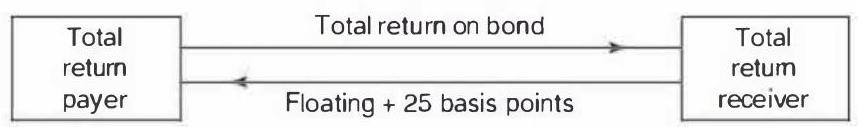
\includegraphics[width=0.7\textwidth]{images/0196660e-d86d-7ef6-8951-a48e2a482302_57_395_444_858_127_0.jpg}
\end{center}
\hspace*{3em} 

The payer:转嫁市场风险和信用风险

The receiver: 获得融资， 融资成本是 floating rate+ spread

\begin{itemize}
\item 原版书例题: a total return swap is a 5-year agreement with a notional principal of \$100 million to exchange the total return on a corporate bond for the floating rate plus 25 basis points.
\end{itemize}

 期间:

The payer: 支付 coupons

The receiver: 支付 floating rate+ 25 bps

期末:

如果债券价值增长 \({10}\%\) : The payer pays \({100}\mathrm{\;m} \times  {10}\%  = {10}\mathrm{\;m}\)

如果债券价值降低 15\%: The receiver pays \({100}\mathrm{\;m} \times  {15}\%  = \$ {15}\mathrm{\;m}\)

债券违约:TRS 停止， receiver 支付债券市场价格和\$100 million 的差额





\subsection{Structured credit products CR-22}

1. 资产证券概述

\begin{itemize}
\item securitisation 证券化过程将贷款或应收款等资产(叫做 collateral or securitized assets)的所有权从原始所有者转移到一个特殊法律实体 (SPV/SPE)。然后， SPV 发行证券， 利用资产产生的现金流向投资者支付利息和偿还本金。这些证券统称为资产支持证券(asset-backed securities， ABS) - 资产证券化过程
\end{itemize}

\begin{center}
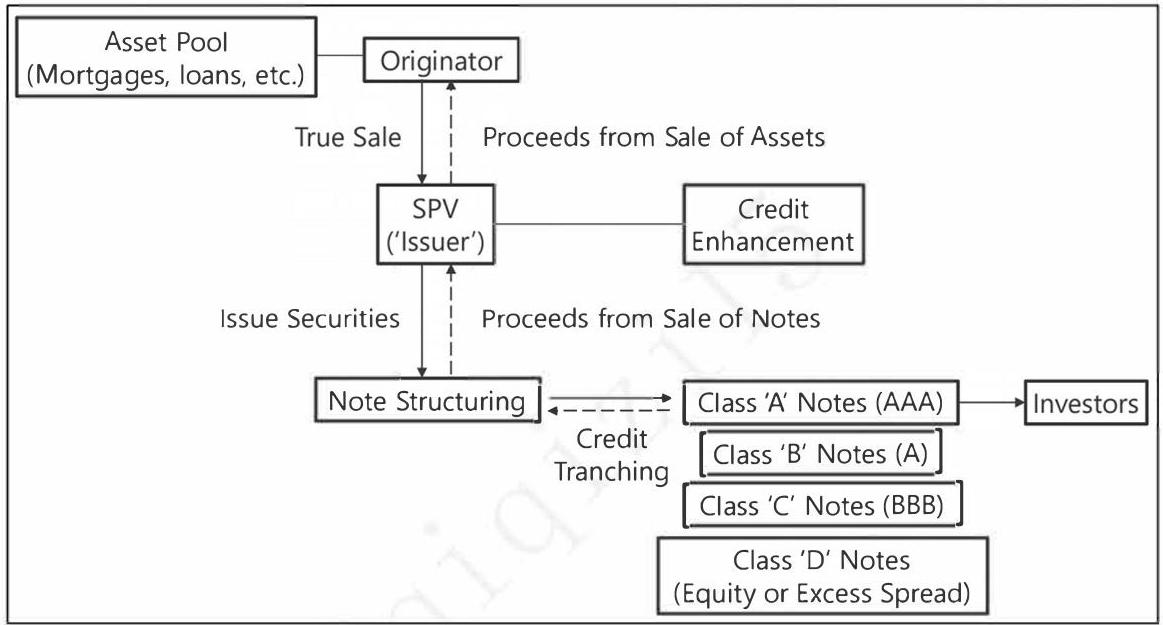
\includegraphics[width=0.9\textwidth]{images/0196660e-d86d-7ef6-8951-a48e2a482302_58_309_659_1163_625_0.jpg}
\end{center}
\hspace*{3em} 

\begin{itemize}
\item 证券化的参与者
\end{itemize}

发起人 (sponsor， seller)。

the entity whose assets are being securitized.

The loan originator is the original lender who creates the debt obligations in the collateral pool， often a bank.

一般是银行

I Issuer (underwriter， arranger， SPV): is set up specially for the purpose of securitization.

Aggregates the underlying loans， designs the securitization structure and markets the liabilities.

Warehousing risk 仓储风险: risk that deal will not be completed and value of accumulated collateral falls. 【产品无法完成或没卖出去， 且已积累的抵押品价值下跌的风险。】

’评级机构(rating agencies)，为证券化产品评定信用评级。

Rating agencies are compensated by issuers， creating a potential conflict

 服务机构和管理机构(servicers and managers):服务和管理资产池的机构。

比较复杂的证券化产品，需要专人进行管理，比如 CDO

 托管人和监管机构(trustee and custodian)，对账户或者标的资产进行管理的机构。

\begin{itemize}
\item 资产证券化的动机【主要从银行和投资者角度分析】
\end{itemize}

融资 Funding

Banks can use securitisation to:

(i) support rapid asset growth 支持资产快速增长;

(ii) diversify their funding mix and reduce cost of funding 多样化融资来源并降低融资成本；

(iii) reduce maturity mismatches 减少期限错配

Balance Sheet Capital Management 资产负债资本管理

Banks use securitisation to improve balance sheet capital management.This provides:

regulatory capital relief 监管资本减免: 通过证券化减轻银行的资本要求。

economic capital relief 经济资本减免；

diversified sources of capital 多样化资本来源: 证券化作为传统资本筹集的替代

Risk Management 风险管理

减少信用风险暴露: 资产出售给 SPV， 降低或完全移除银行的信用风险。

剥离不良资产:移除不良资产和负面情绪，同时释放监管资本。 对投资者的好处

diversify sectors of interest;

access different (and sometimes superior) risk-reward profiles;

access sectors that are otherwise not open to them.

\begin{itemize}
\item SPV Structures
\end{itemize}

 按照证券化产品的结构可将其分为不同的类别。主要有以下分类:

摊销结构 Amortizing structures(pass-through structure): pay principal and interest to investors on a coupon-by-coupon basis throughout the life of the security.在证券的整个存续期间按期支付本金和利息给投资者。

比如常见的 MBS

They are priced and traded based on expected maturity and weighted-average life (WAL)【基于 WAL 定价与交易】

* weighted-average life (WAL): 即本金未偿还的时间加权时间

\begin{itemize}
\item WAL \(= \sum \frac{\text{ Actual Days }}{365} *\) Pool factor
\end{itemize}

Pool factor: 池因子， is the repayment weighting adjustment to the notional value outstanding \(\left( {\mathrm{O}/\mathrm{S}}\right)\) 【会给出】

A WAL approach incorporates various pre-payment assumptions， and any change in this pre-payment speed will increase or decrease the rate at which principal is repaid to investors.【WAL 方法包含各种提前还款假设】

循环结构(revolving structures):使资产本金循环流转。这种结构适用于像信用卡贷款或者汽车贷款。这类贷款的期限通常期限较短且提前还款速度较快，其现金流划分为两个期限，分别是循环期和摊销期。

During the revolving period 循环期， principal collections are used to purchase new receivables that fulfil the necessary criteria. 【收到的本金用于购买符合条件的新应收账款】

During the amortisation period 摊销期， principal payments are paid to investors either in a series of equal installments (controlled amortisation) or the principal is "trapped' in a separate account until the expected maturity date and then paid in a single lump sum to investors (soft bullet). 【在摊销期，本金可以通过等额分期付款或在到期日一次性支付的方式支付给投资者。】

综合信托 (master trust): 指证券化产品是根据投资者需求灵活设计的， 既可以构建摊销结构，也可以构建循环结构。

Frequent issuers under US and UK law use master trust structures， which allow multiple securitisations to be issued from the same SPV。

Under such schemes， the originator transfers assets to the master trust SPV. Notes are then issued out of the asset pool based on investor demand. 【发起人将资产转移到 master trust SPV， 然后根据投资者的需求从资产池中发行票据。】

Master trusts are used by MBS and credit card ABS originators.

2. asset pools

\begin{itemize}
\item Classifications of asset pools
\end{itemize}

\begin{itemize}
\item 根据资产类别:
\end{itemize}

 债权类资产

Auto loans 汽车贷款

Credit card 信用卡

Mortgage 住房贷款

Debt obligation

 Loan pool: 比如某个游乐场的门票收益，打包发行证券化产品

\begin{itemize}
\item By type of pools
\end{itemize}

\begin{itemize}
\item Static pools 静态池: are amortizing pools in which a fixed loans is placed in the trust. 【资产池的资产是固定的， 比如 100 个贷款， 假设 4 个违约， 那么资产池还剩 96 个贷款】
\end{itemize}

E.g.: auto loans and residential mortgages.

Revolving pools 循环池: specify an overall level of assets to be maintained during a revolving period. As underlying loans are repaid， the size is maintained by introducing additional loans from the balance sheet of the originator.

E.g.: credit card debt.

Managed pool 管理池 \(s\) : manager of the structured product has discretion to remove individual loans from the pool， and replace them with others. 【移除池中的个别贷款， 并用其他贷款替换】

E.g.: CDOs.

\begin{itemize}
\item 证券化产品主要受资产池的影响。因此在评估证券化产品的风险时， 我们要更加关注标的资产池的 performance measure。【这个表格虽然是截图的， 但是有几个指标需要重点掌握: 比如 CPR、WAL、DSCR。下面给了几个例题可以做一做感受一下】
\end{itemize}

\begin{center}
\adjustbox{max width=\textwidth}{
\begin{tabular}{|c|c|c|}
\hline
Performance Measure & Calculation & Typical Asset Class \\
\cline{1-3}
Public Securities Association (PSA) & PSA = [CPR/(.2)(months)]*100 & mortgages， home-equity， student loans \\
\cline{1-3}
Constant prepayment rate (CPR) & \(1 - {\left( 1 - \mathrm{{SMM}}\right) }^{12}\) & mortgages， home-equity. student loans \\
\cline{1-3}
Single monthly mortality (SMM) & Prepayment/Outstanding pool balance & mortgages， home-equity， student loans \\
\cline{1-3}
Weighted average life (WAL) & \(\sum\) (a/365).PF(s) Where \(\mathrm{{PF}}\left( \mathrm{s}\right)\) & mortgages \\
\cline{1-3}
Weighted average maturity (WAM) & Weighted maturity of the pool & mortgages \\
\cline{1-3}
Weighted average coupon (WAC) & Weighted coupon of the pool & mortgages \\
\cline{1-3}
Debt service coverage ratio (DSCR) & Net operating income/Debt payments & commercial mortgages \\
\cline{1-3}
Monthly payment rate (MPR) & Collections/Outstanding pool balance & all non-amortising asset classes \\
\cline{1-3}
Default ratio & Defaults/Outstanding pool balance & credit cards \\
\cline{1-3}
Delinquency ratio & Delinquents/Outstanding pool balance & credit cards \\
\cline{1-3}
Absolute prepayment speed (ABS) & Prepayments/Outstanding pool balance & auto loans， truck loans \\
\cline{1-3}
Loss curves & Show expected cumulative loss & auto loans， truck loans \\
\cline{1-3}
\hline
\end{tabular}
}
\end{center}

Example 1 : Given an ABS with total outstanding balance of credit card receivables of \$57，800，000. \$900，000 are over 90 days past due. Additionally， \(\$ 1，{200}，{000}\) of receivables were written off. Total monthly principal and interest payments per month are \(\$ 1，{580}，{000}\) . Calculate the delinquency ratio， default ratio， and monthly payment rate for this ABS.

Delinquency Ratio \(= \$ {900}，{000}/\$ {57}，{800}，{000} = {1.577}\%\)

Default Ratio \(= \$ 1，{200}，{000}/\$ {57}，{800}，{000} = {2.076}\%\)

Monthly Payment Rate (MPR) \(= \$ 1，{580}，{000}/\$ {57}，{800}，{000} = {2.734}\%\)

Example 2: Suppose an MBS has net operating income from commercial mortgaged properties equal to \(\$ {89}，{572}，{500}\) . The total debt payments for notes issued against these mortgages is equal to \(\$ {87}，{958}，{000}\) . Calculate the debt service coverage ratio (DSCR).

DSCR \(= \$ {89}，{572}，{500}/\$ {87}，{958}，{000} = {1.02}\)

Example 3 : Suppose an MBS is composed of three different pools of mortgages: \(\$ 6\) million of mortgages that yield 7.8\%， \$10 million of mortgages that yield \({6.0}\%\) ， and \(\$ 4\) million of mortgages that yield 5\%. Calculate the weighted average coupon (WAC).

WAC \(= 6/\left( {6 + {10} + 4}\right)  \times  {7.8}\%  + {10}/\left( {6 + {10} + 4}\right)  \times  6\%  + 4/\left( {6 + {10} + 4}\right)  \times  5\%  = {6.34}\%\)

Example 4 : Given an MBS composed of 3 different pools of mortgages: \(\$ 2\) million of mortgages with a maturity of 180 days， \$6 million of mortgages with a maturity of 360 days， and \$12 million of mortgages with a maturity of 90 days. Calculate the WAM.

WAM \(= 2/\left( {2 + 6 + {12}}\right)  \times  {180} + 6/\left( {2 + 6 + {12}}\right)  \times  {360} + {12}/\left( {2 + 6 + {12}}\right)  \times  {90} = {180}\)

 Example 5: Given an ABS with an SMM of 1.2\%. This implies that the approximate prepayment for the month is equal to 1.2\% of the remaining mortgage balance for the month less the scheduled principal repayment. Calculate the CPR for this MBS.

CPR \(= 1 - {\left( 1 - {1.2}\% \right) }^{12} = {0.1349}\)

\section*{3. Structured products}

\begin{center}
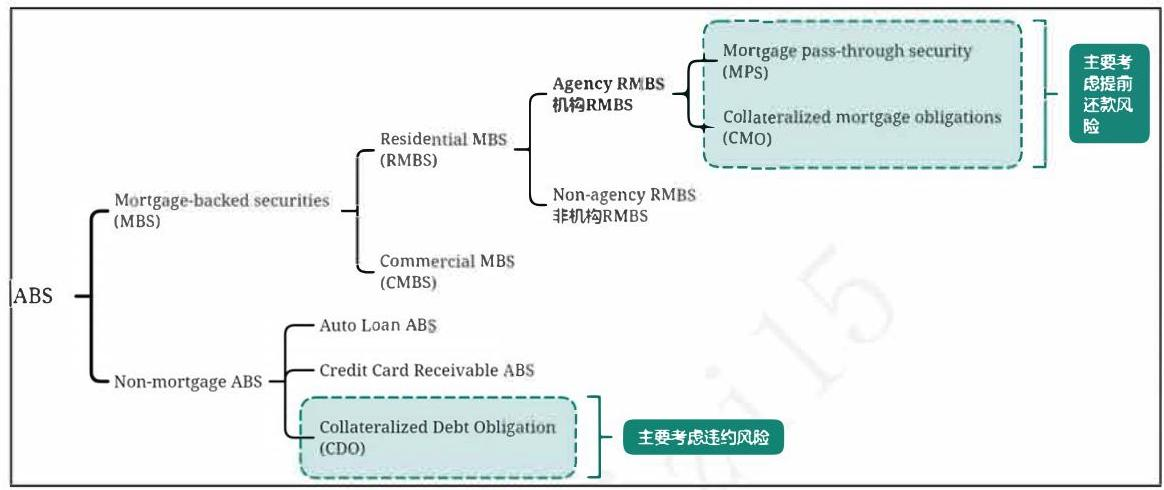
\includegraphics[width=0.9\textwidth]{images/0196660e-d86d-7ef6-8951-a48e2a482302_63_239_605_1164_490_0.jpg}
\end{center}
\hspace*{3em} 

(1) mortgage pass-through security (MPS)

\begin{itemize}
\item The simplest agency MBSs are pass-throughs。
\end{itemize}

\begin{itemize}
\item 所有的投资者拿到 same return. 投资者每个月拿到的现金流来源于借款人每月归还的房贷。其中包括利息、本金以及提前归还(prepayment)的本金。
\end{itemize}

(2) Collateralized mortgage obligations (CMOs) 担保抵押债券

\begin{itemize}
\item 对于抵押资产池或者 MPS 的现金流， 进行重新分配， 以形成不同 tranche。 不同的 tranche 会有不用的风险和收益， 以满足不同投资者的需求。这样形成的证券， 叫做 CMO.
\end{itemize}

\begin{itemize}
\item CMO 的产生并不能消除而只是转移提前还款风险。【我们这里介绍的是机构 MBS，信用风险比较小，提前还款风险比较大。所以，这里的分层主要针对的是提前还款风险的再分配】
\end{itemize}

(3) 担保债务凭证(Collateralized Debt Obligation， CDO)

\begin{itemize}
\item 抵押资产: a diversified pool of one or more debt obligations
\end{itemize}

 种类:

\begin{center}
\adjustbox{max width=\textwidth}{
\begin{tabular}{|c|c|}
\hline
名称 & 抵押资产 \\
\cline{1-2}
collateralized bond obligations (CBOs) & corporate and emerging market bonds \\
\cline{1-2}
collateralized loan obligations & leveraged bank loans \\
\cline{1-2}
\hline
\end{tabular}
}
\end{center}

\begin{center}
\adjustbox{max width=\textwidth}{
\begin{tabular}{|c|c|}
\hline
(CLOs) & \phantom{X} \\
\cline{1-2}
structured finance CDOs & ABS， RMBS， CMBS， and other CDOs \\
\cline{1-2}
synthetic CDOs & a portfolio of credit default swaps for other structured securities \\
\cline{1-2}
\hline
\end{tabular}
}
\end{center}

\begin{itemize}
\item 根据信用风险可以分为: senior， mezzanine， and equity tranches.
\end{itemize}

高级层(senior tranche):违约风险最小，收益最小-最安全

 夹层 (mezzanine tranche) : 违约风险和收益居中

 股权层(equity tranche):违约风险最大，收益最大-一般发行人自留；

 如果贷款人违约，首先损失的 equity tranche，其次是 mezzanine tranche， 最后是 senior tranche

\begin{itemize}
\item Credit enhancement 信用增强
\end{itemize}

有些证券化产品信用风险比较大，会采用一些手段让这些产品看起来更好看(风险小)。这些手段中， 其中常用的是 Credit enhancement 信用增强。

The lower the quality of the assets being securitized， the greater the need for credit enhancement. 具体而言有: 超额抵押(overcollateralization)

post more collateral than is needed to obtain or secure financing. 实际发行的证券化产品的规模小于资产的规模。

比如贷款资产池规模是 100million，发行面值 90million 的证券化产品

超额利差 (excess spread)

贷款资产池收到的的现金流大于支付的证券化产品的利息。【后面会更详细的介绍】

资产池保险 (pool insurance) 购买保险， 如果贷款资产池违约， 保险公司给与赔付

分层(subordination):划分偿付的优先顺序，对最高层级产品进行信用增级。

逐渐上升的利息(margin step-up)

\begin{itemize}
\item PD and Default Correlation
\end{itemize}

 【底层资产池的违约，以及违约相关性，是影响证券化产品风险的关键因素。 我们这里从资产池角度讨论】

Increasing Default Probability (Correlation Constant)

\begin{center}
\adjustbox{max width=\textwidth}{
\begin{tabular}{|c|c|c|}
\hline
\phantom{X} & Mean Value & Credit VaR \\
\cline{1-3}
Equity tranche & ↓ & ↓ \\
\cline{1-3}
Mezzanine tranche & ↓ & \(\uparrow\) then \(\downarrow\) \\
\cline{1-3}
Senior tranche & ↓ & ↑ \\
\cline{1-3}
\hline
\end{tabular}
}
\end{center}

Increasing Correlations (Default Probability Constant)

\begin{center}
\adjustbox{max width=\textwidth}{
\begin{tabular}{|c|c|c|}
\hline
\phantom{X} & Mean Value & Credit VaR \\
\cline{1-3}
Equity tranche & ↑ & ↑ \\
\cline{1-3}
Mezzanine tranche & (at low default rates) \(\uparrow\) (at high default rates) & ↑ \\
\cline{1-3}
Senior tranche & ↓ & ↑ \\
\cline{1-3}
\hline
\end{tabular}
}
\end{center}

Default'01

 Default'01 用于衡量当PD变动一个基点时，对于证券化产品价值的影响。 通常以违约概率每上升或下降 10 个基点为整体衡量对于证券化产品价值的影响:

\[
\text{ Default’01 } = \frac{1}{20}\lbrack \text{ (mean value/loss based on }\pi  + {0.001}\text{ ) } -
\]

\[
\text{ (mean value/loss based on }\pi  - {0.001}\text{ )] }
\]

\begin{itemize}
\item CDO 的种类
\end{itemize}

 现金型 CDO(cash CDO):最传统的 CDO

合成型 CDO(synthetic CDO):卖出 CDS 和买入无风险资产共同构成资产证券化产品

 单一层级 CDO(single-tranche CDO):所发行的证券化产品只有一个层级【为了满足投资者的定制化需求】。

通常不会直接收购资产池，而是类似合成 CDO 一样，通过 CDS 构造。 4. Cash waterfall 现金流瀑布

\begin{itemize}
\item 现金流瀑布分析: all the cash that is generated by the asset pool is paid in order of payment priority.
\end{itemize}

The senior debt receives all of its promised payments before any lower tranche receives any monies.

我们这里分析的不是摊销结构(amortizing structure)，也就是前期只有利息， 最后一期还本付息。【和普通债券一样的现金流结构】

\section*{资产池现金流流入 cash inflow=Aggregate loan interest received+Recovery amount}

Aggregate loan interest received 利息部分

Recovery amount 有些资产会违约， 违约时的回收部分

最后一期的本金

\begin{itemize}
\item 资产池现金流流出 cash outflow=Bond coupon interest due to both the junior and senior bonds.
\end{itemize}

\begin{itemize}
\item Overcollateralization account (OC)超额抵押账户:像一个蓄水池， 把多余的资金存起来， 以备不时之需。
\end{itemize}

包含三部分资金:

Excess spread: Excess spread=资产池 Cash Inflows-Cash outflows

每年存入的 Excess spread 会有上限， 多余的就给到 equity 层

有些资产池违约时的 Recovery amount

之前年份的 OC earn the financing money market rate of \(\mathrm{r}\) 。即之前年份的 OC 的利息

\begin{itemize}
\item 原版书例题:
\end{itemize}

Imagine a CLO， the underlying assets of which are 100 identical leveraged loans， with a par value of \(\$ 1，{000}，{000}\) each， and priced at par. The loans are floating rate obligations that pay an annual coupon of fixed spread of 3.5 percent over Libor. Assume there are no upfront， management， or trustee fees. The maturity of underlying assets is five-year and the maturity of CLO is five-year.

\begin{itemize}
\item Capital structure displayed in this schematic balance sheet:
\end{itemize}

Senior tranche: 本金\$85 million; coupon rate= L+50 bps

Mezz Tranche: 本金 \$10 million; coupon rate=L+500bps

Equity Tranche: 本金 \$5 million;

 问题 1. If defaults happen， PD=2\%， RR=40\%. Given N= 100， K(存入 Excess spread 的上限) \(= \$ {1.75}\) million， Libor \(= 5\%\) .please define the coupon cash flow of CLO for the five years.

\begin{center}
\adjustbox{max width=\textwidth}{
\begin{tabular}{|c|c|c|c|c|c|c|c|c|c|c|}
\hline
1 t & 2 Def & 3 Cum & 4 Srv & 5 Loan int & 6 Exc spr & 700 & 8 Recov & 90C+ Recov & 10 Eq flow & 11 OC a/c \\
\cline{1-11}
1 & 2 & 2 & 98 & 8，330，000 & 2，655，000 & 1，750，000 & 800，000 & 2，550，000 & 905，000 & 2，550，000 \\
\cline{1-11}
2 & 2 & 4 & 96 & 8，160，000 & 2，485，000 & 1，750，000 & 800，000 & 2，550，000 & 735，000 & 5，227，500 \\
\cline{1-11}
\hline
\end{tabular}
}
\end{center}

\begin{center}
\adjustbox{max width=\textwidth}{
\begin{tabular}{|c|c|c|c|c|c|c|c|c|c|c|}
\hline
3 & 2 & 6 & 94 & 7，990，000 & 2，315，000 & 1，750，000 & 800，000 & 2，550，000 & 565，000 & 8，038，875 \\
\cline{1-11}
4 & 2 & 8 & 92 & 7，820，000 & 2，145，000 & 1，750，000 & 800，000 & 2，550，000 & 395，000 & 10，990，819 \\
\cline{1-11}
5 & 2 & 10 & 90 & 97，650，000 & \phantom{X} & \phantom{X} & 800，000 & 800，000 & - & 11，540，360 \\
\cline{1-11}
\hline
\end{tabular}
}
\end{center}

Key to columns:

(1)Year index

(2)Number of defaults during year \(t\)

(3) Cumulative number of defaults， at the end of year t

(4) Number of surviving loans， at the end of year t

(5) Loan interest

(6)Excess spread

(7)Overcollateralization increment

(8)Recovery amount Rt

(9) Aggregate flow into overcollateralization account \(\mathrm{{OCt}} + \mathrm{{Rt}}\)

(10) Interim cash flow to the equity at the end of year \(t\) .

(11) The value of the overcollateralization account at time t.

 分析:

第一年: 资产池中的 100 个贷款有 2 个违约， 剩余 98 个未违约

Loan int \(= {98}，{000}，{000} \times  {8.5}\%  = 8，{330}，{000}\)

3 支付给最高层级和中间层级支付的利息总额为 5，675，000

Senior tranche:85million \(* \left( {5\%  + {0.5}\% }\right)  = 1\) million

Mezz Tranche:10million \(* \left( {5\%  + 5\% }\right)  = {4.675}\) million

Total cash outflow \(= 1\mathrm{{million}} + {4.675}\mathrm{{million}} = 5，{675}，{000}\)

Exc spr=8，330，000-5，675，000=2，655，000

其中 1，750，000 美元放入 OC

剩余的 905，000 美元给 equity

OC+ Recov=1，750，000+2*1000000*40\%=2，550，000

OC a \(/c = 2，{550}，{000}\)

第二年: 剩余 96 个未违约

Loan int \(= {96}，{000}，{000} \times  {8.5}\%  = 8，{160}，{000}\)

3 支付给最高层级和中间层级支付的利息总额为 5，675，000

Senior tranche:85million \(* \left( {5\%  + {0.5}\% }\right)  = 1\) million

Mezz Tranche:10million \(* \left( {5\%  + 5\% }\right)  = {4.675}\) million

Total cash outflow \(= 1\mathrm{{million}} + {4.675}\mathrm{{million}} = 5，{675}，{000}\)

Exc spr=8，160，000-5，675，000=2，485，000

其中 1，750，000 美元放入 OC

剩余的 735，000 美元给 equity



\hspace*{5em} * OC+ Recov=1，750，000+2*1000000*40\%=2，550，000

* OC a/c=2，550，000*(1+5\%)+2，550，000=5，227，500



\begin{itemize}
\item 依次可得第三年和第四年。
\end{itemize}

第五年: 利息和本金

4 剩余 90 个未违约

* Loan 本息和(cash inflow)=90，000，000*(1+8.5\%)=97，650，000

总计: \({97}，{650}，{000} + {10}，{990}，{819}^{ * }\left( {1 + 5\% }\right)  + {800}，{000} = {109}，{990}，{360}\)

outflow=85 million*(1+5\%+0.5\%)+10

million* \(\left( {1 + 5\%  + 5\% }\right)  = {100}，{675}，{000}\)

* 109，990，360 > 100，675，000 ， 因此在最后一年 Senior 和 Mezz 的投资者可以得到自己应得的资金

* 而 equity 投资者可得 109，990，360-100，675，000=9315360

 问题 2:If defaults happen， PD=10\%， RR=40\%. Given N= 100， K(存入 Excess spread 的上限)=\$1.75million， Libor=5\%.please define the coupon cash flow of CLO for the five years.

\begin{center}
\adjustbox{max width=\textwidth}{
\begin{tabular}{|c|c|c|c|c|c|c|c|c|c|c|}
\hline
1 t & 2 Def & 3 Cum & 4 Srv & 5 Loan int & 6 Exc spr & 700 & 8 Recov & 90C+ Recov & 10 Eq flow & \({11}\mathrm{{OCa}}/\mathrm{c}\) \\
\cline{1-11}
1 & 10 & 10 & 90 & 7，650，000 & 1，975，000 & 1，750，000 & 4，000，000 & 5，750，000 & 225，000 & 5，750，000 \\
\cline{1-11}
2 & 9 & 19 & 81 & 6，885，000 & 1，210，000 & 1210，000 & 3，600，000 & 4，810，000 & 0 & 10，847，500 \\
\cline{1-11}
3 & 8 & 27 & 73 & 6，205，000 & 530，000 & 530，000 & 3，200，000 & 3，730，000 & 0 & 15，119，875 \\
\cline{1-11}
4 & 7 & 34 & 66 & 5，610，000 & -65，000 & -65，000 & 2，800，000 & 2，735，000 & 0 & 18，610，869 \\
\cline{1-11}
5 & 7 & 41 & 59 & 64，015，000 & \phantom{X} & \phantom{X} & 2，800，000 & 2，800，000 & \phantom{X} & 19，541，412 \\
\cline{1-11}
\hline
\end{tabular}
}
\end{center}

第一年: 资产池中的 100 个贷款有 10 个违约， 剩余 90 个未违约

Loan int \(= {90}，{000}，{000} \times  {8.5}\%  = 7，{650}，{000}\)

支付给最高层级和中间层级支付的利息总额为 5，675，000

Senior tranche:85million \(* \left( {5\%  + {0.5}\% }\right)  = 1\) million

Mezz Tranche:10million \(* \left( {5\%  + 5\% }\right)  = {4.675}\) million

Total cash outflow \(= 1\mathrm{{million}} + {4.675}\mathrm{{million}} = 5，{675}，{000}\)

Exc spr=7，650，000-5，675，000=1，975，000

其中 1，750，000 美元放入 OC

剩余的 225，000 美元给 equity

OC+ Recov=1，750，000+10*1000000*40\%=5，750，000

\begin{itemize}
\item \(\mathrm{{OCa}}/\mathrm{c} = 5，{750}，{00}\)
\end{itemize}

第二、三年分析方式一样

第四年， cash outflow 大于 cash inflow， 因此 Exc spr 小于零， 从 OC 中拿出一分部给到 Senior 和 Mezz 的投资者。

第五年: 还利息和本金

4 剩余 59 个未违约

* Loan 本息和(cash inflow)=59，000，000*(1+8.5\%)=64，015，000

* 18，610，869*(1+5\%)+2，800，000=19，541，412

* 总计: \({64}，{015}，{000} + {18}，{610}，{869} * \left( {1 + 5\% }\right)  + 2，{800}，{000} = {86356412}\)

* Total cash outflow \(= {85}\) million \({}^{ * }\left( {1 + 5\%  + {0.5}\% }\right)  + {10}\) million \({}^{ * }\)  \(\left( {1 + 5\%  + 5\% }\right)  = {89675000} + {11000000}\)

* 86，356，412 < 89675000 ，因此在最后一年 Senior、Mezz 和 equity 都遭受损失
